\clearpage
\subsection{Expressions (with Function Calls, Variables, and Constants)} % (fold)
\label{sub:expressions_with_variables_}

You can \textbf{read} the values from Variables and Constants within Expressions. The value of the expression is calculated by \textbf{reading} the values from the Variables and Constants when the expression is calculated\footnote{This means that the value will be affected by the statements that occurred before the expression was calculated.}.

\begin{figure}[h]
   \centering
   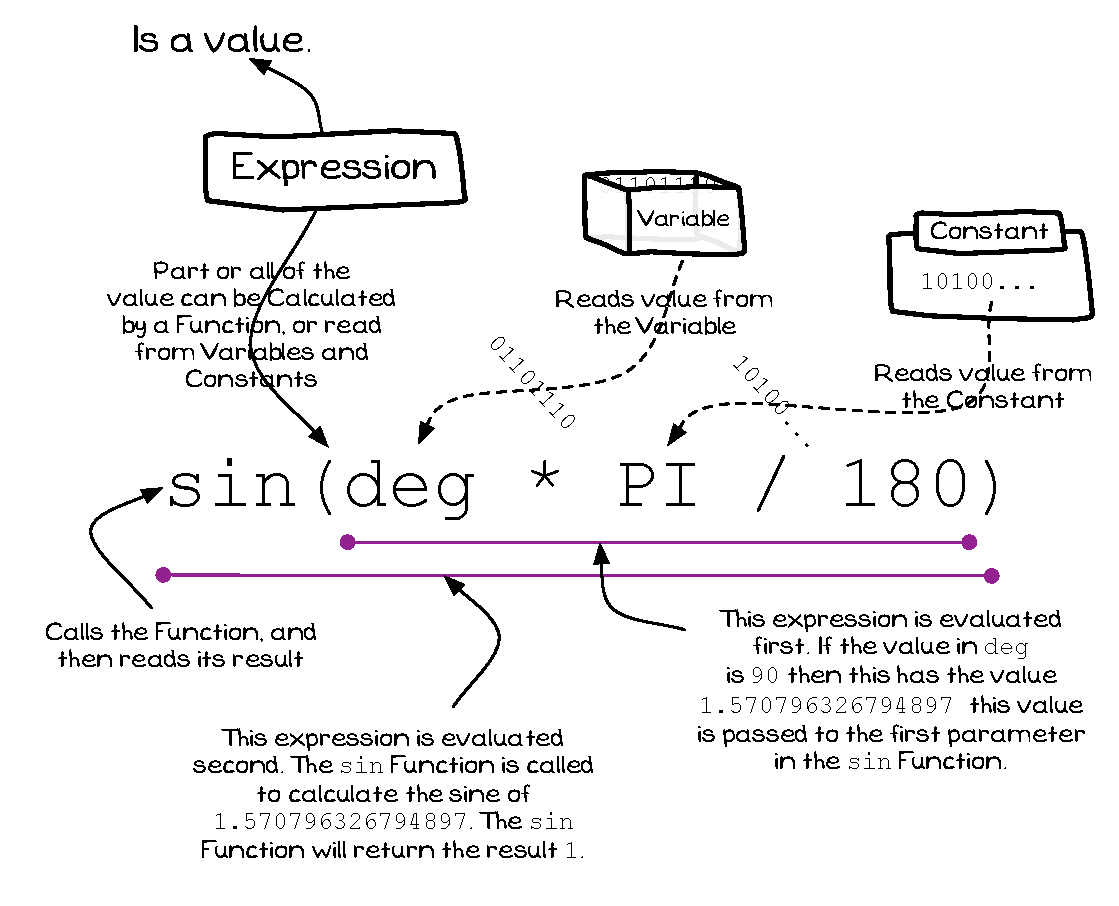
\includegraphics[width=0.9\textwidth]{./topics/storing-using-data/diagrams/Expression} 
   \caption{Expressions can read values from Function Calls, Variables, and Constants}
   \label{fig:expressions-with-variables}
\end{figure}

\mynote{
\begin{itemize}
  \item Expression is the \textbf{term} given to the code that calculates values within your Statements.
  \item You can read values from Function Calls, Variables, and Constants.
  \item You use the Variable or Constant's name to access its value within an Expression.
  \item The \nameref{sub:function_call} runs the code in the Function, and then reads the result returned.
  \item There are actually \textbf{two expressions} in Figure \ref{fig:expressions-with-variables}:
  \begin{enumerate}
    \item The first Expression is the value passed to the \texttt{sin} function (\texttt{$deg \times PI \times 180$}). This value is calculated by reading the values from the \texttt{deg} variable and the \texttt{PI} constant. These values are then used in the Expression to determine that value that is passed to the Parameter in \texttt{sin}.
    \item The second Expression is the result returned from the call to the \texttt{sin} function. This will calculate the sine of the value calculated in the first expression.
  \end{enumerate} 
  \item The Expression reads the value of the Variable \textbf{at the time} it is executed.
  \item Expressions are used to calculate values that are...
  \begin{itemize}
    \item Passed to Parameters within \nameref{sub:procedure call}s.
    \item Assigned to Variables within \nameref{sub:assignment_statement}s.
  \end{itemize}
\end{itemize}
}


% subsection expressions_with_variables_ (end)